\chapter[Modelado de Requerimientos]{Modelado de Requerimientos}
\label{cp:modelling}

\parindent0pt

El modelado de requerimientos constituye la etapa inicial del lado izquierdo del modelo en V, que enfatiza la importancia de las pruebas en cada fase del ciclo de vida del proyecto de software. El objetivo principal de esta etapa es comprender, documentar y validar las necesidades y expectativas de los actores interesados del sistema, definiendo de forma precisa su comportamiento y funcionalidades. Esta fase se asocia directamente con las pruebas de aceptación del lado derecho de la V, la etapa final del modelo, en la cual se verifica que el sistema cumple con los requerimientos definidos inicialmente.

El modelado de requerimientos incide directamente en las etapas subsiguientes de diseño, implementación y pruebas. Los errores o ambigüedades en la fase de modelado pueden propagarse a lo largo del proyecto, resultando en un aumento del tiempo y los recursos requeridos para corregirlos. Por lo tanto, la inversión de esfuerzo para asegurar que los requerimientos sean claros, completos y factibles reduce el riesgo de inconsistencias y la necesidad de refactorizaciones en fases posteriores, contribuyendo a la ejecución exitosa del proyecto.

En el contexto del desarrollo de un prototipo de aplicación con tecnología blockchain para la trazabilidad y valorización de envases de vidrio, el modelado de requerimientos busca garantizar que el prototipo responda a las necesidades específicas de una \gls{economiacircular} sostenible y transparente. Con este objetivo, el proceso de modelado se estructuró en una serie de pasos iterativos para descubrir, definir y refinar los requerimientos del sistema. En la Figura \ref{fig:requirements-modelling-process}, se pueden observar las etapas del proceso, las cuales comprenden: definición de dominio, de casos de uso, de requerimientos y de historias de usuario.

\begin{figure}[!htb]
    \centering
    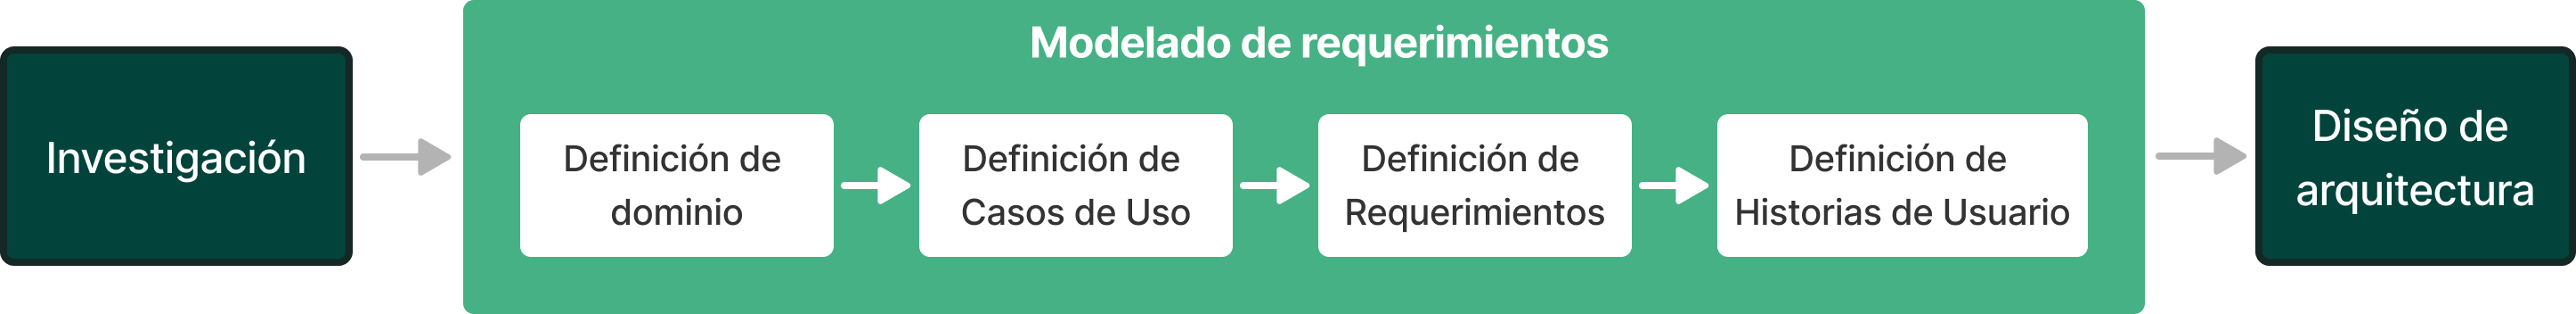
\includegraphics[width=\linewidth]{Figures/requirements-modelling.png}
    \caption{Etapas del proceso de modelado de requerimientos del prototipo de trazabilidad de vidrio}
    \label{fig:requirements-modelling-process}
\end{figure}

El proceso dio inicio con una investigación exhaustiva del dominio del problema para identificar los actores clave y sus interacciones (Sección \ref{sec:domain-definition}). A partir de esta información, se elaboró una propuesta de valor para documentar las necesidades y expectativas de cada actor junto con posibles soluciones. Posteriormente, se modelaron los casos de uso para describir las funcionalidades del sistema desde la perspectiva del usuario (Sección \ref{sec:use-cases}). Estos casos de uso constituyeron la base para la definición formal de los requerimientos funcionales y no funcionales, incluyendo sus interdependencias (Sección \ref{sec:requirements-definition}). Finalmente, se redactaron \textit{historias de usuario} con un nivel de detalle suficiente para definir los criterios de aceptación, lo cual permitió iniciar las etapas de diseño de arquitectura, estimación de esfuerzo y planificación de la implementación.

\section{Definición de Dominio}
\label{sec:domain-definition}

El modelado de requerimientos inicia con la definición del dominio del problema. En el contexto de este proyecto, que busca la trazabilidad y valorización del vidrio, el objetivo es comprender el entorno en el que el sistema operará, identificando los actores y sus interacciones. El análisis establece la base para la construcción de los requerimientos del sistema.

La definición del dominio se realizó a través de una investigación y revisión de la literatura sobre la \gls{trazabilidad} del vidrio. En la Sección \ref{sec:related-work}, se exploraron los trabajos existentes en el área de blockchain aplicada para lograr una economía circular, también se investigaron proyectos existentes que aborden la misma temática o el uso de tecnología para el mismo fin. A su vez, se realizaron entrevistas e investigaciones de campo con expertos en la industria del vidrio y el reciclaje regional, para comprender los procesos actuales, las problemáticas y las expectativas de los actores involucrados (Apéndices \ref{cp:verallia-interview} y \ref{cp:europe-trip}). Se examinaron las etapas del ciclo de vida de los envases de vidrio, desde su producción hasta su reintroducción en la cadena de valor, para identificar los puntos donde la tecnología blockchain puede aplicarse. La Figura \ref{fig:glass-lifecycle-modelling} ilustra el ciclo de vida de los envases de vidrio y los actores involucrados en cada etapa.

\begin{figure}[!htb]
    \centering
    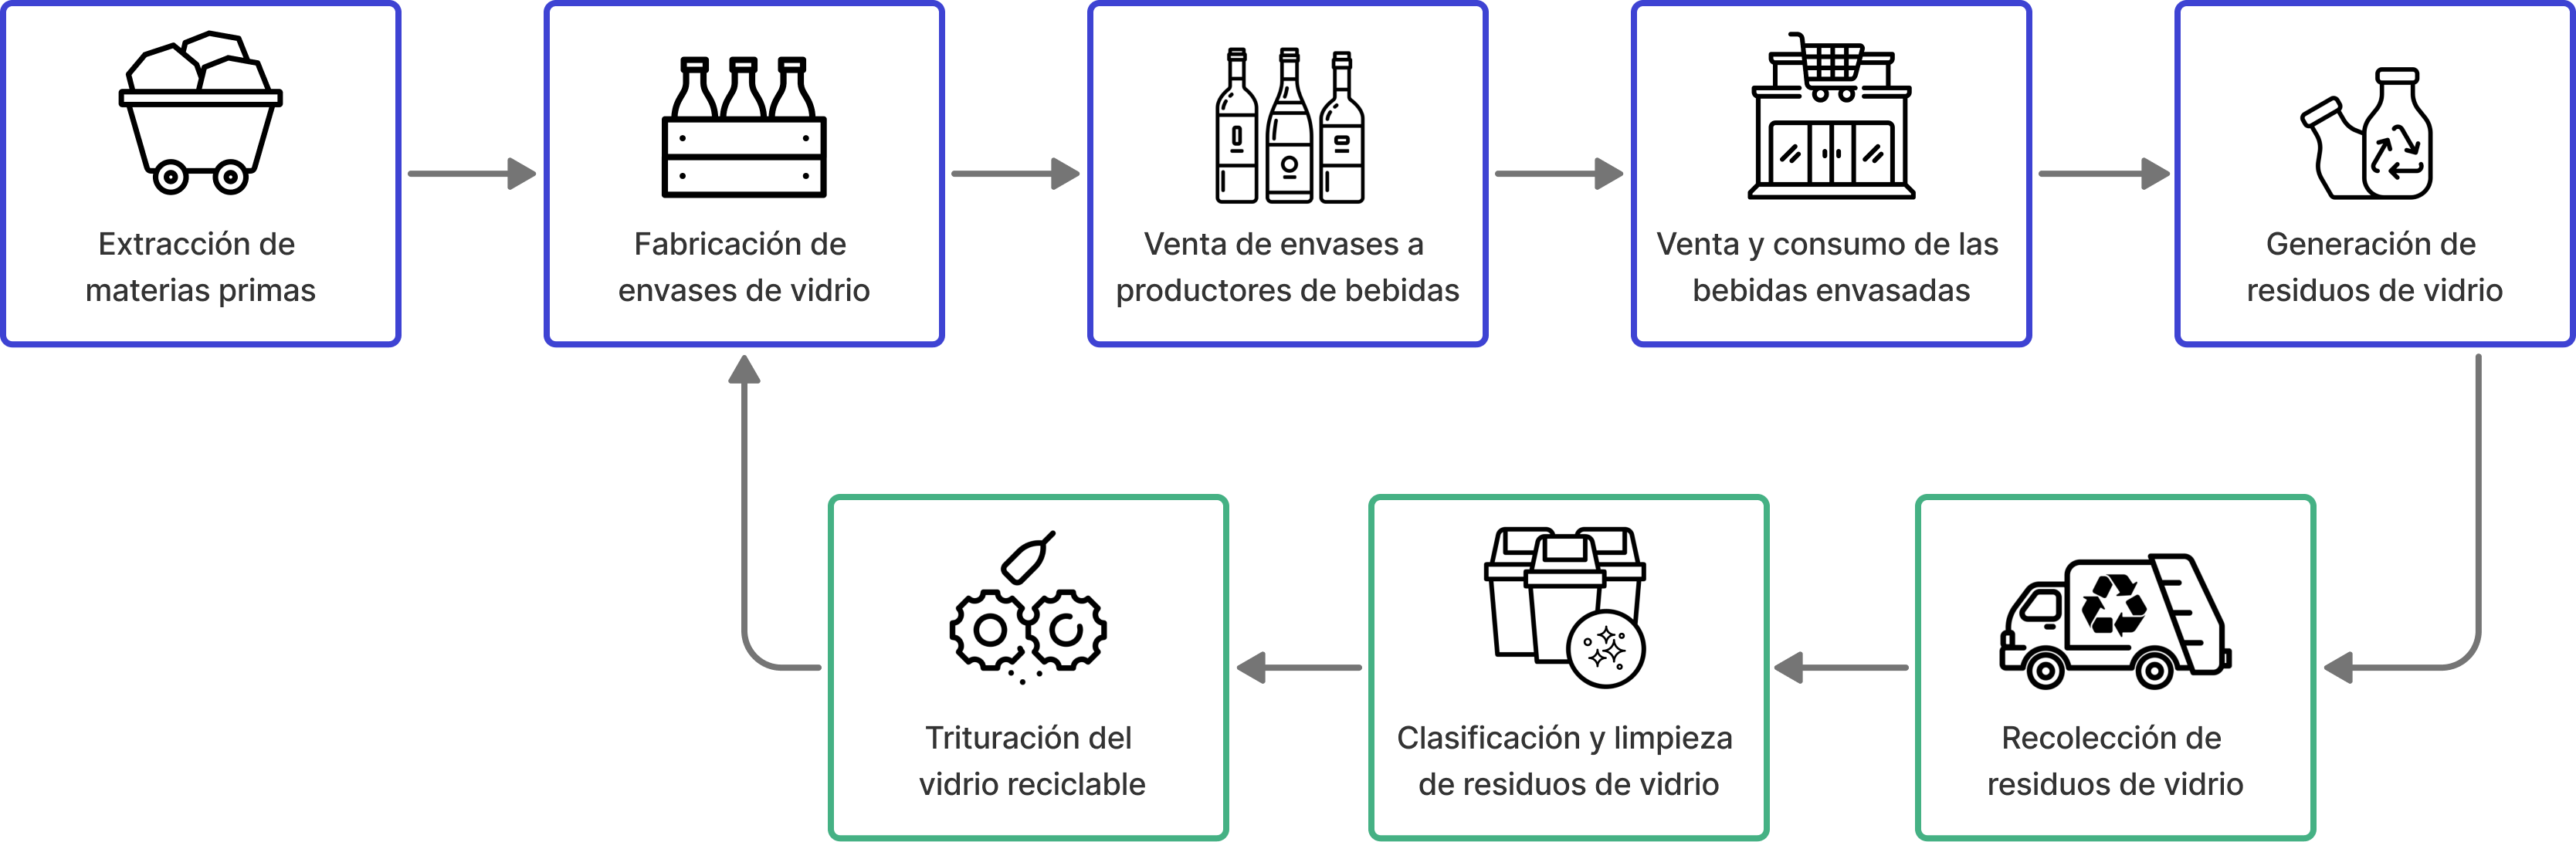
\includegraphics[width=\linewidth]{Figures/glass-lifecycle.png}
    \caption{Etapas del ciclo de vida de los envases de vidrio}
    \label{fig:glass-lifecycle-modelling}
\end{figure}

En este marco, se identificaron los siguientes actores clave:

\begin{itemize}
    \item \textbf{Productor de Vidrio (Productor Primario):} Fabricante del envase de vidrio, con la responsabilidad de registrar la información inicial del lote de material.
    \item \textbf{Productor de vino (Productor Secundario):} Empresa productora de vino que utiliza el envase de vidrio para embotellar sus productos y requiere acceder a la información de trazabilidad con el fin de garantizar la calidad y seguridad alimentaria.
    \item \textbf{Consumidor:} Usuario final que adquiere bebidas envasadas, las consume y puede participar en el proceso de reciclaje.
    \item \textbf{Centro de Reciclaje:} Entidad que recibe, procesa y recicla el vidrio, utiliza la información de trazabilidad para verificar la calidad del material reciclado y dejar registro de su disposición final.
\end{itemize}

Dado que el público objetivo del sistema incluye a todos los actores involucrados en la cadena de valor de los envases de vidrio, se planteó realizar una propuesta de valor que incluya a todos ellos, teniendo en cuenta sus procesos, necesidades y expectativas sobre una solución tecnológica. Para ello, se utilizó la herramienta \textit{canvas de propuesta de valor} \footnote{\url{https://www.interaction-design.org/literature/topics/value-proposition-canvas}}, un diagrama semi-estructurado que permite documentar de manera flexible las necesidades y problemáticas de cada actor, facilitando la comprensión de sus expectativas. Esta herramienta suele ser utilizada por empresas y diseñadores de forma estratégica para analizar, evaluar y ajustar la propuesta de valor de su producto o servicio para alinearla con las necesidades de sus clientes.

Un canvas de propuesta de valor se divide en dos secciones principales: el perfil del actor y el mapa de valor de la solución. En el perfil del actor, se detallan sus necesidades, deseos y miedos, lo que proporciona una visión clara de sus motivaciones y los obstáculos que enfrentan en su estado actual. En el mapa de valor de la solución, se definen las funcionalidades y experiencia que ofrecerá la solución, con el objetivo de aplacar los miedos y satisfacer las necesidades y los deseos de los actores. Este análisis conjunto de las expectativas y la solución permite adoptar un enfoque centrado en el usuario desde el inicio del proceso de diseño de solución, asegurando que el sistema responda directamente a las problemáticas identificadas.

La propuesta de valor de la solución de trazabilidad se analiza a través de cuatro canvas de propuesta de valor, elaborados para cada uno de los actores clave de la cadena. Este análisis sirve como el primer paso para conceptualizar cómo el sistema basado en blockchain puede mitigar los problemas existentes y generar valor tangible para cada participante. El canvas de propuesta de valor para el Productor Primario de vidrio (Figura \ref{fig:value-proposition-canvas-primary-producer}) y el del Productor Secundario de bebidas (Figura \ref{fig:value-proposition-canvas-secondary-producer}) ilustran las necesidades de estos actores, focalizándose en sus responsabilidades y objetivos empresariales, mientras que la solución aborda sus desafíos logísticos y de \gls{sostenibilidad}. Por su parte, la Figura \ref{fig:value-proposition-canvas-consumer} presenta el canvas para el Consumidor, centrando el análisis en su rol como punto de partida para el reciclaje. Finalmente, la Figura \ref{fig:value-proposition-canvas-recycler} muestra el canvas para el Centro de Reciclaje, detallando cómo la solución puede optimizar sus procesos de clasificación y venta de materiales.

\begin{figure}[!htb]
    \centering
    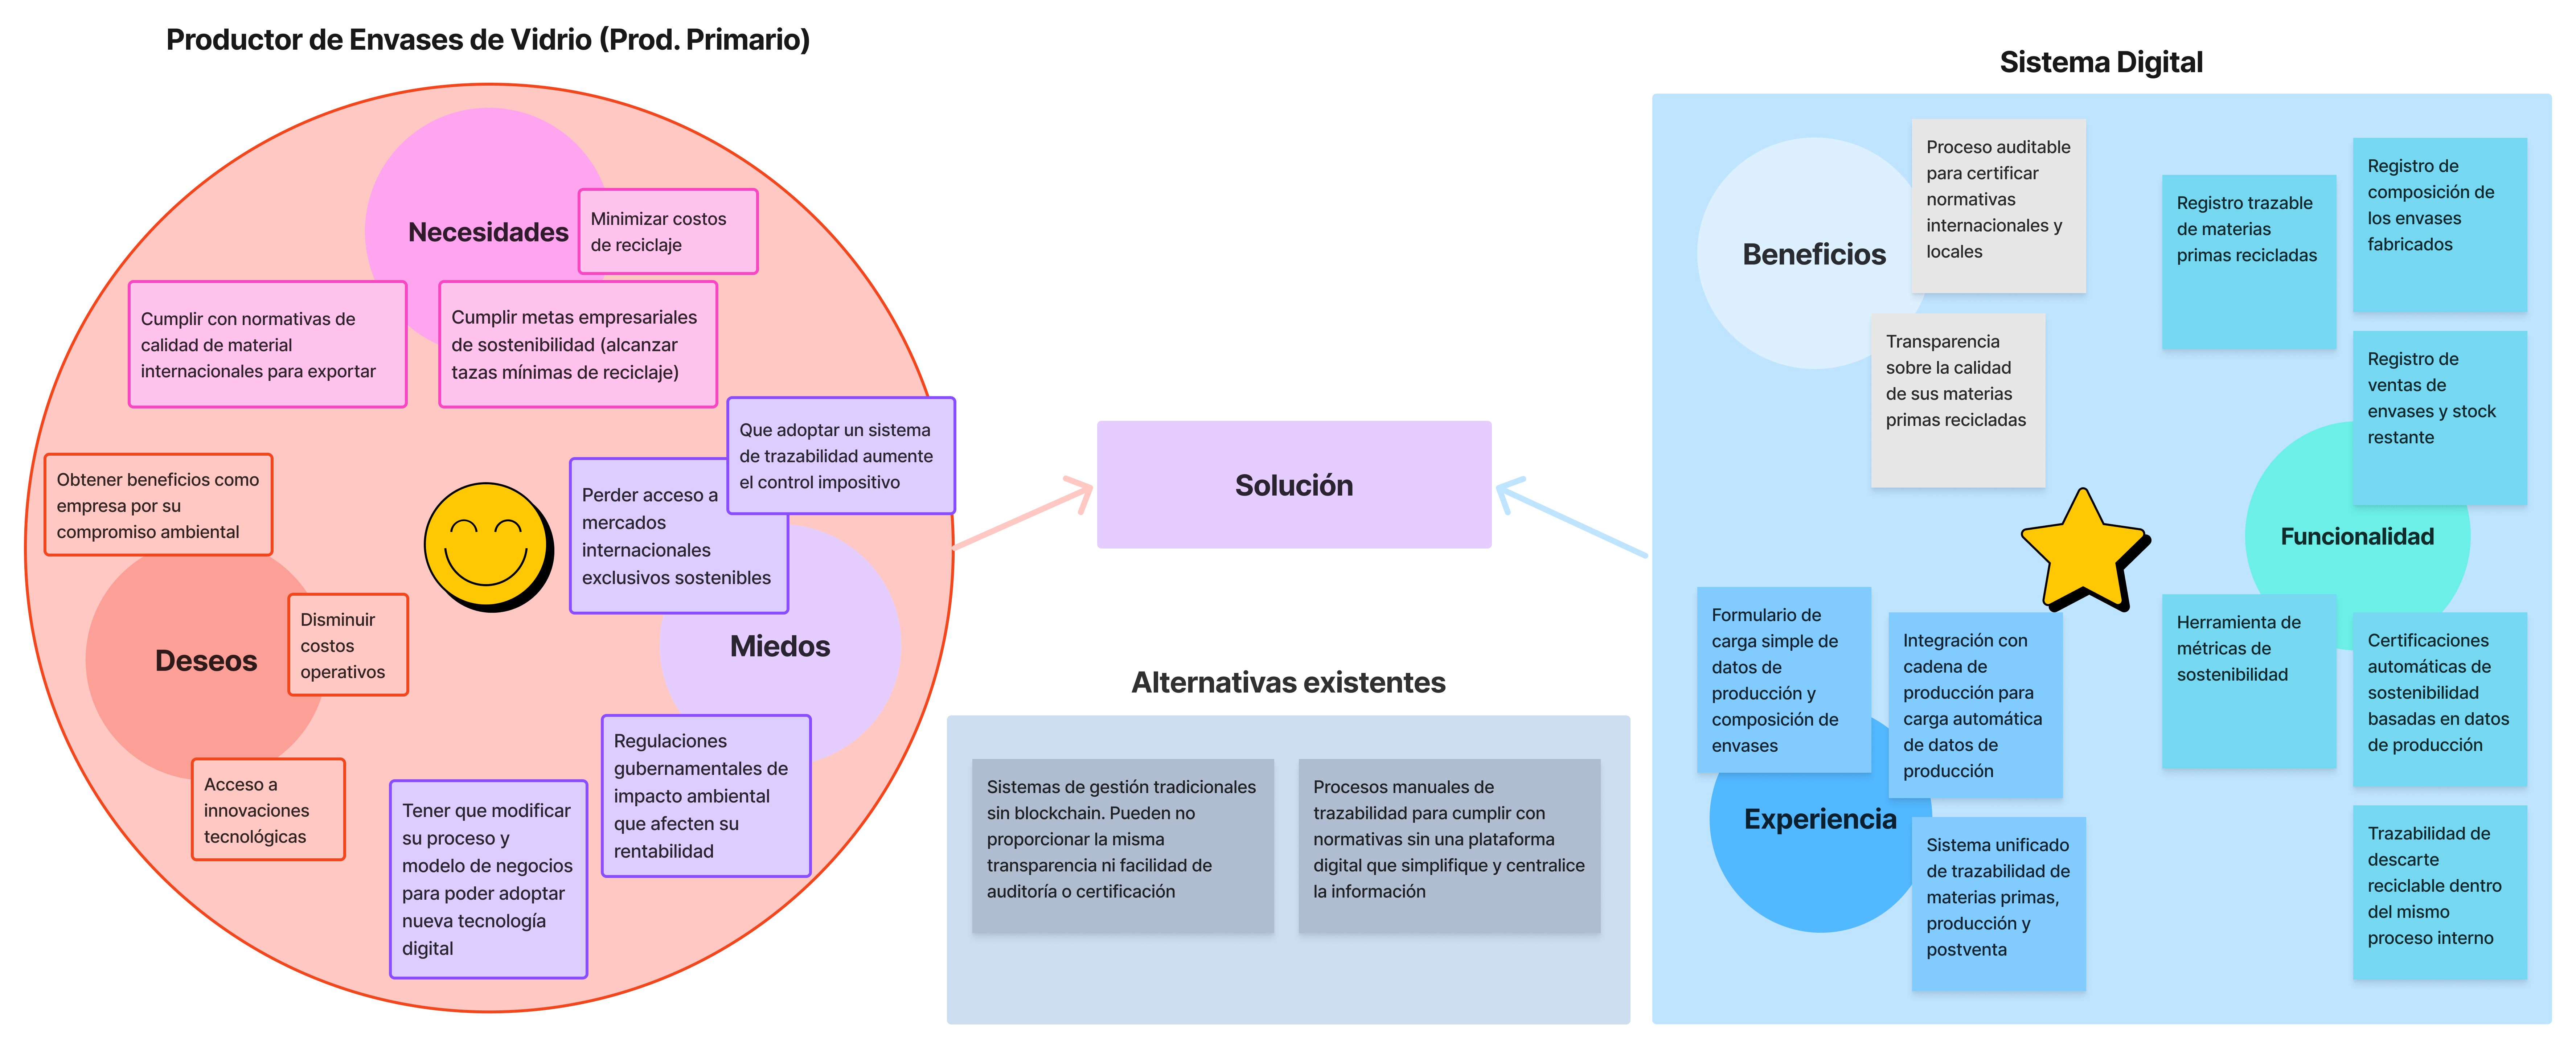
\includegraphics[width=\textwidth]{Figures/value-proposition-canvas-primary-producer.png}
    \caption{Canvas de propuesta de valor para el Productor Primario de vidrio}
    \label{fig:value-proposition-canvas-primary-producer}
\end{figure}

\begin{figure}[!htb]
    \centering
    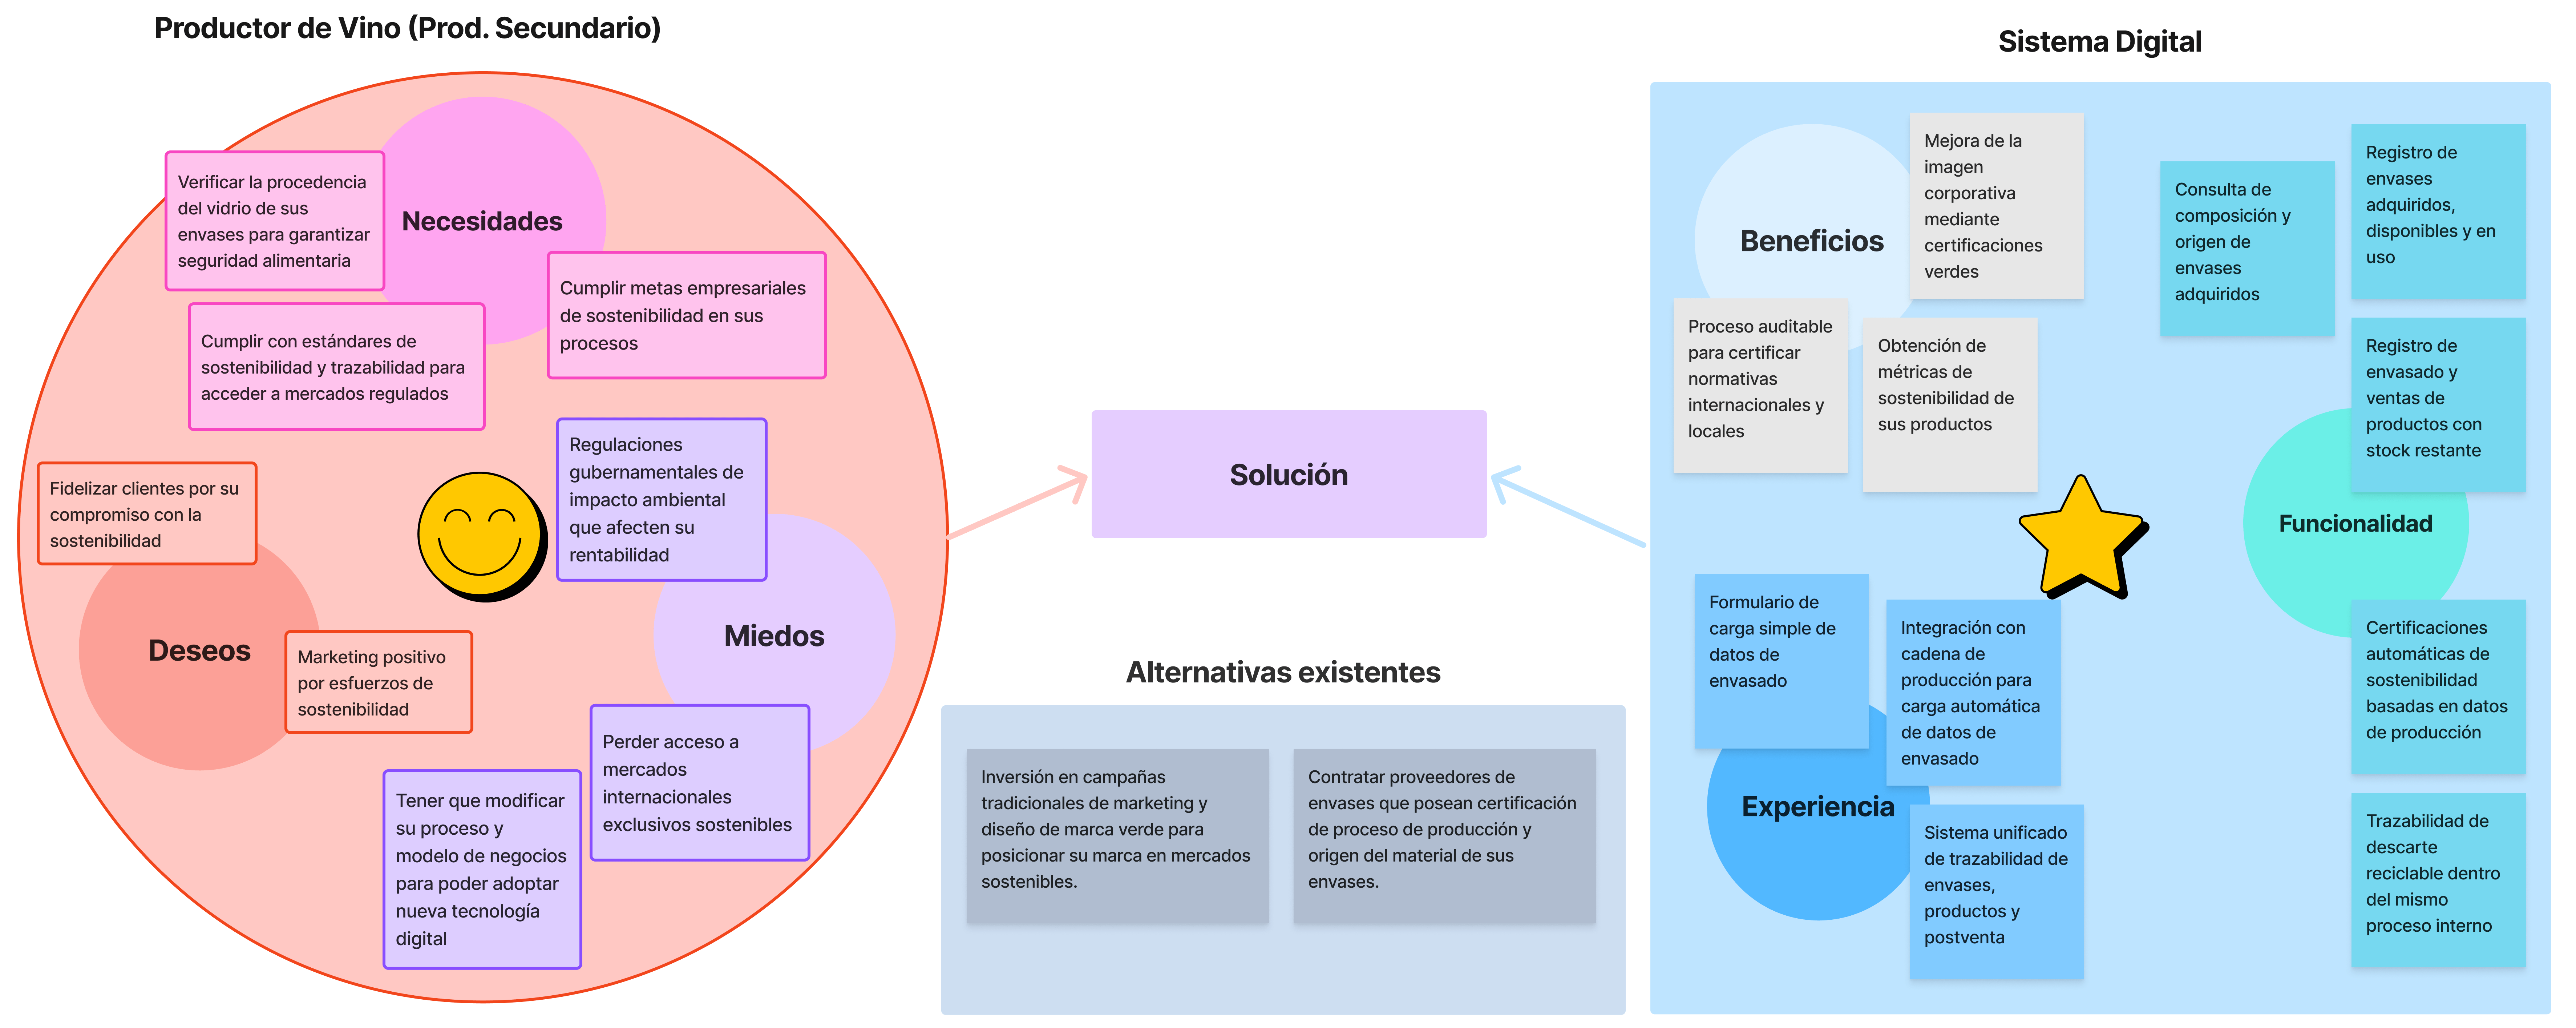
\includegraphics[width=\textwidth]{Figures/value-proposition-canvas-secondary-producer.png}
    \caption{Canvas de propuesta de valor para el Productor Secundario de bebidas}
    \label{fig:value-proposition-canvas-secondary-producer}
\end{figure}

\begin{figure}[!htb]
    \centering
    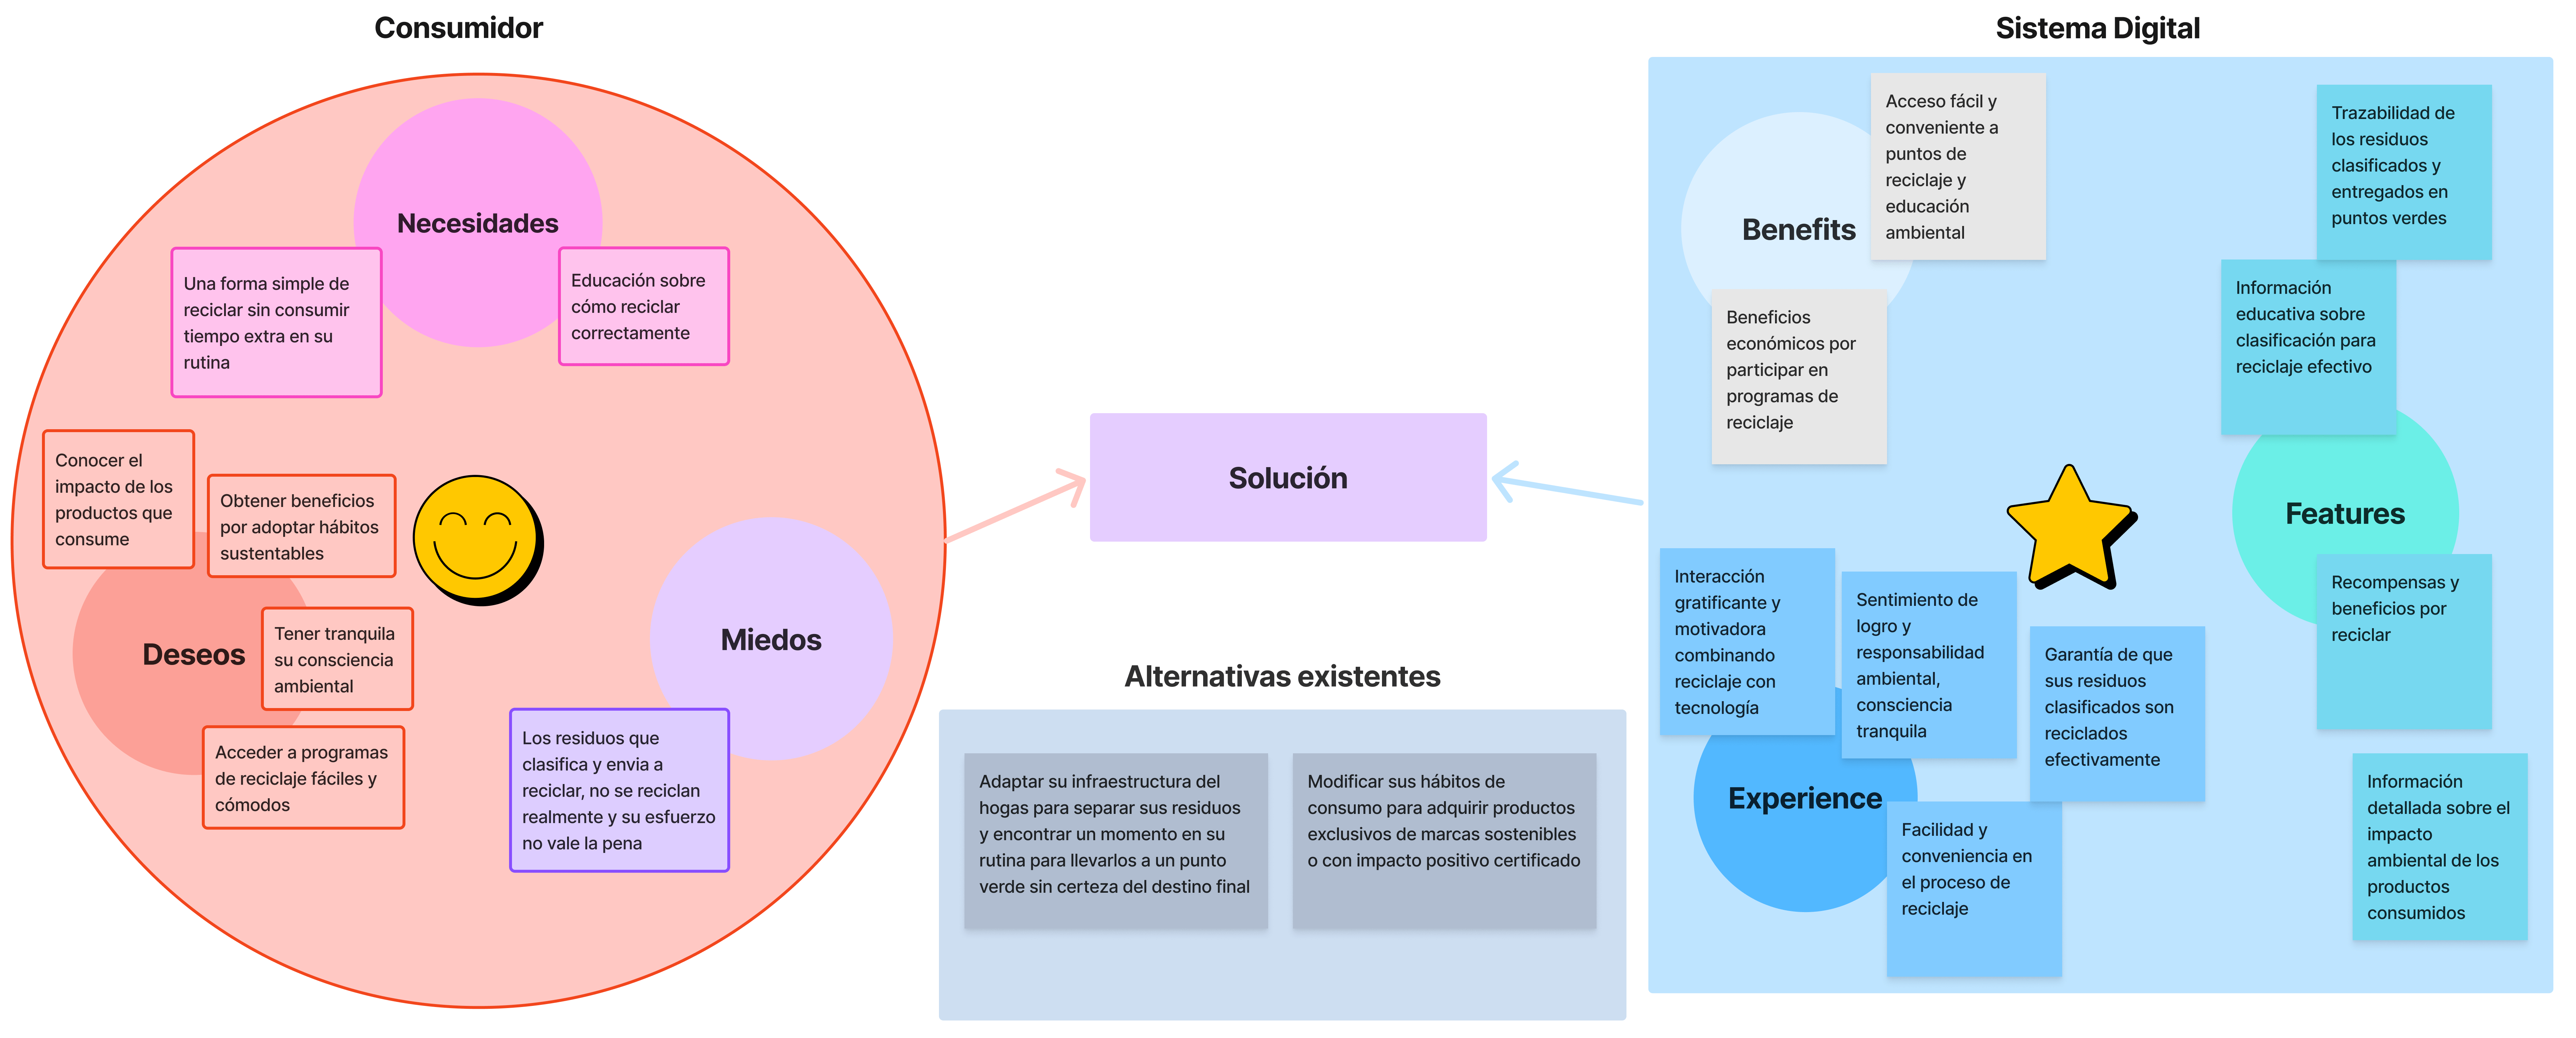
\includegraphics[width=\textwidth]{Figures/value-proposition-canvas-consumer.png}
    \caption{Canvas de propuesta de valor para el Consumidor}
    \label{fig:value-proposition-canvas-consumer}
\end{figure}

\begin{figure}[!htb]
    \centering
    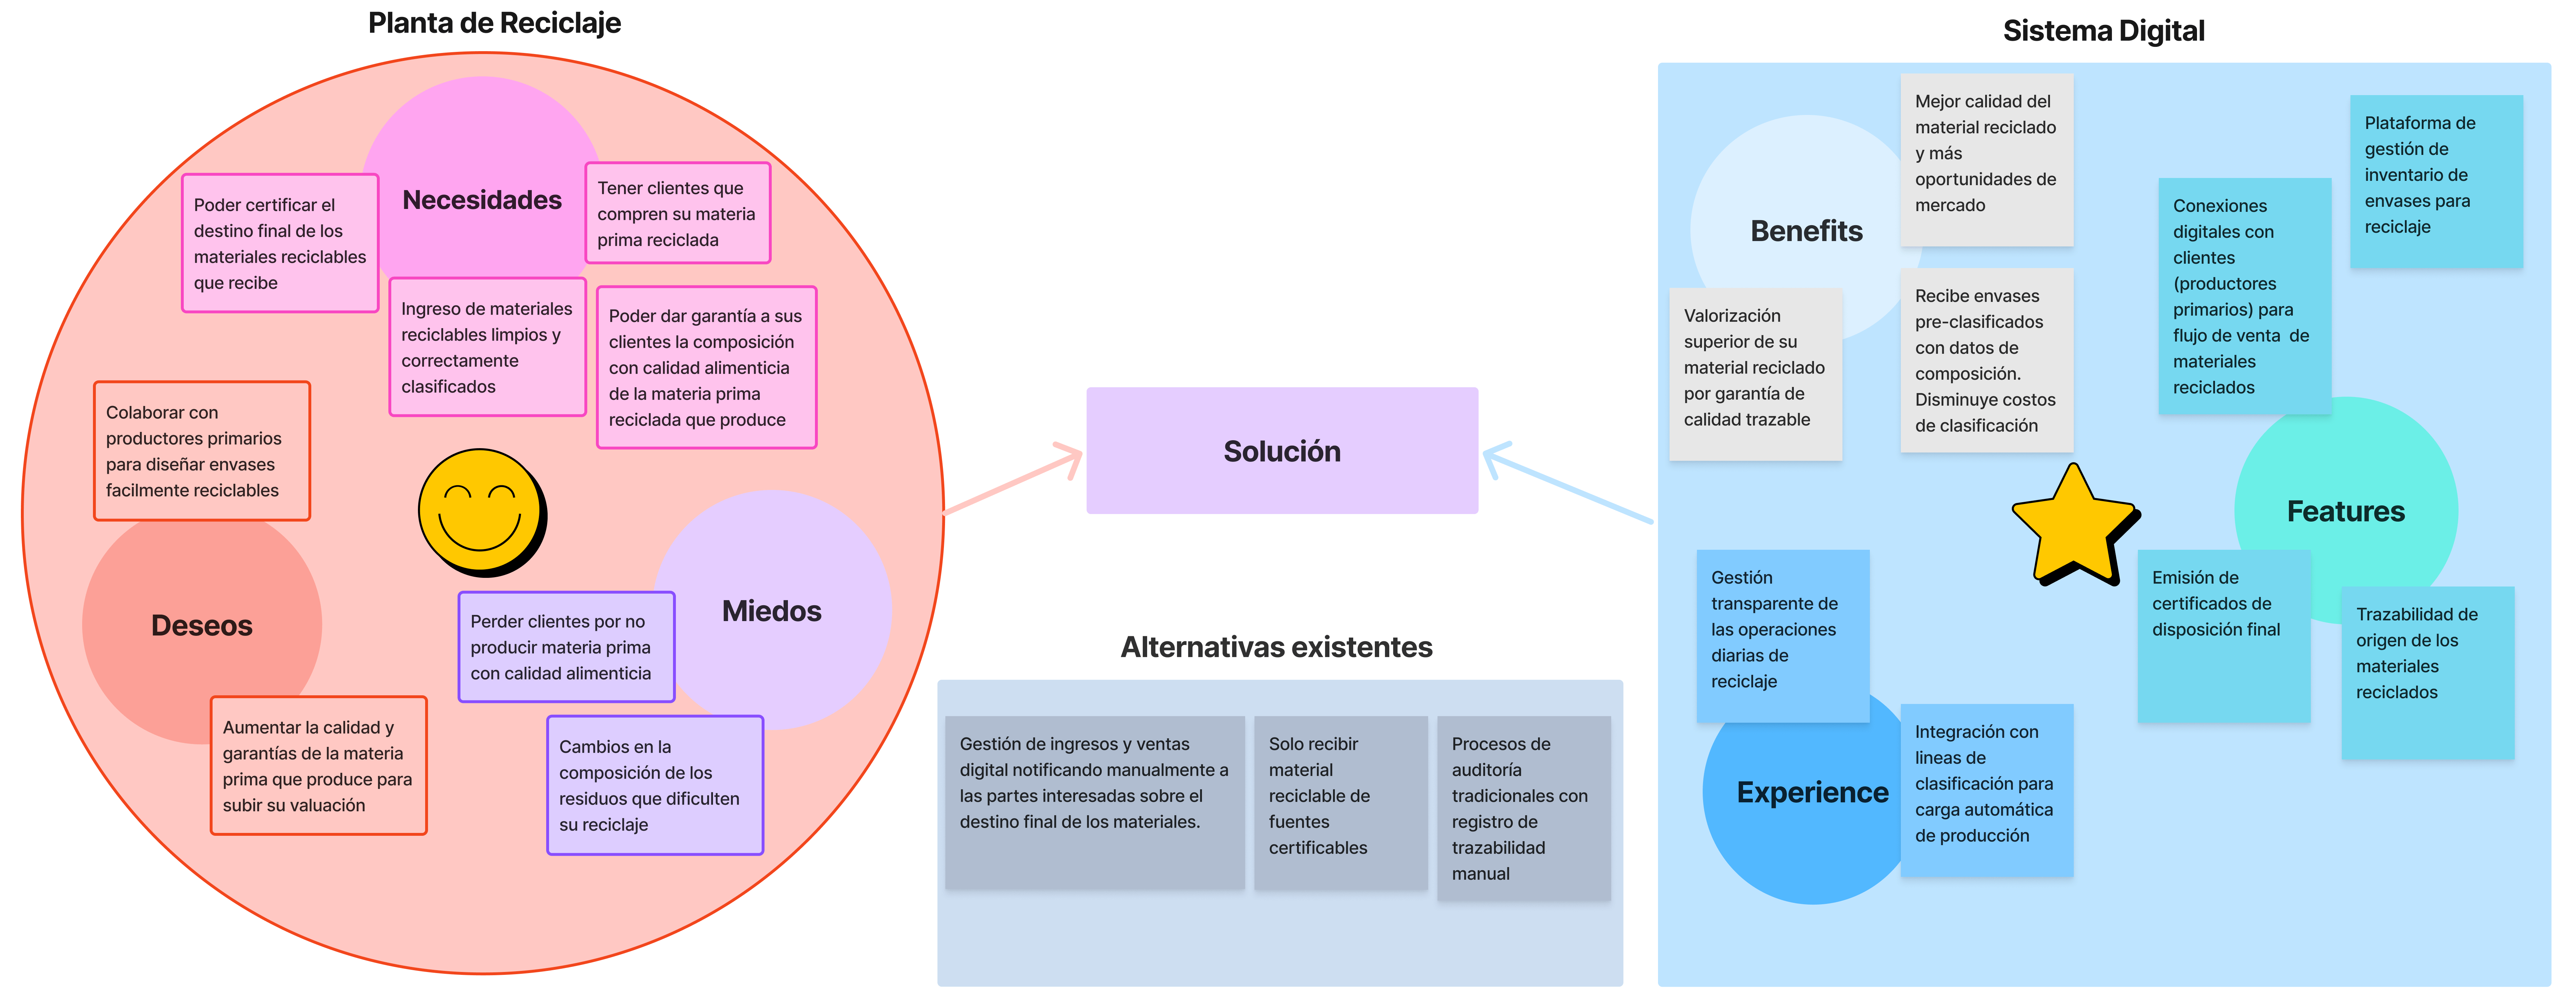
\includegraphics[width=\textwidth]{Figures/value-proposition-canvas-recycler.png}
    \caption{Canvas de propuesta de valor para el Centro de Reciclaje}
    \label{fig:value-proposition-canvas-recycler}
\end{figure}

El análisis detallado a través del canvas de propuesta de valor revela que los principales desafíos se centran en la falta de transparencia y la ineficiencia de los procesos actuales involucrados en el ciclo de vida del vidrio. El Productor Primario necesita un flujo constante de materia prima reciclada de calidad para minimizar sus costos y cumplir con metas de sostenibilidad. A su vez, el Productor Secundario enfrenta el desafío de verificar la procedencia de los envases de vidrio para garantizar la seguridad alimentaria y, de esta manera, acceder a mercados regulados y sostenibles, cumpliendo sus propias metas de sostenibilidad. Por su parte, el Consumidor busca una forma simple de reciclar, con la seguridad de que su esfuerzo es valorado y recompensado, y desea tener la capacidad de conocer el impacto ambiental de los productos que adquiere. Finalmente, el Centro de Reciclaje se enfrenta a altos costos operativos y a falta de calidad en el material recibido, lo que dificulta su valorización. Estas problemáticas y expectativas compartidas se traducen en la necesidad de un sistema unificado y confiable, que permita a los actores verificar la procedencia del material, documentar cada etapa del ciclo de vida y ofrecer incentivos a los usuarios finales. Por lo tanto, los casos de uso del sistema se diseñan para abordar directamente estas necesidades, permitiendo el registro de lotes de producción de envases, consulta de la trazabilidad de cada unidad, gestión del reciclaje de los envases y verificación de la calidad del material reciclado.

La información recopilada en esta fase proporciona una comprensión de las necesidades de los actores y sienta las bases para la siguiente etapa del modelado de requerimientos, donde se definirán los casos de uso del sistema con una perspectiva centrada en el usuario.

\section{Modelado de Casos de Uso}
\label{sec:use-cases}

Después de definir el dominio y los actores, se procede a la identificación y modelado de los casos de uso. Un caso de uso es una técnica de modelado que describe, de manera detallada y estructurada, las interacciones entre un actor (un usuario o sistema externo) y el sistema para lograr un objetivo de negocio específico. Cada caso de uso representa una funcionalidad completa y significativa desde la perspectiva del usuario, garantizando que el sistema final sea útil para sus usuarios.

El valor de esta herramienta de modelado reside en que permite a los equipos de desarrollo y a los interesados en el negocio comprender el ``qué'' (la funcionalidad), el ``quién'' (el actor) y el ``porqué'' (el objetivo) de cada interacción. Además, facilita la comunicación entre los miembros del equipo y sirve como una base sólida para la identificación de los requerimientos funcionales del sistema, asegurando que el diseño del sistema se alinee con las necesidades reales de los usuarios. Los casos de uso de un sistema se pueden documentar mediante un diagrama de casos de uso, que es una representación gráfica que muestra las relaciones entre los actores y cada caso de uso de forma conjunta, proporcionando una visión general del sistema.

Con el objetivo de acotar el alcance de este trabajo, se realiza el modelado de los casos de uso relacionados con la trazabilidad de los envases de vidrio, abarcando las acciones que los actores pueden realizar en el sistema. Estos casos de uso se centran en las funcionalidades esenciales que permiten a los actores registrar, consultar y gestionar la información relacionada con los envases de vidrio a lo largo de su ciclo de vida. Los casos de uso relacionados con la certificación de cada etapa del proceso e integración con sistemas preexistentes se consideran fuera del alcance de este trabajo, pero los casos de uso modelados permiten sentar las bases para futuras extensiones del sistema hacia estas funcionalidades.

En el prototipo de sistema de trazabilidad para envases de vidrio, los casos de uso comprenden tanto las acciones inherentes al ciclo de vida del material como las interacciones propias de una plataforma digital basada en blockchain. El primer grupo de casos de uso describe las operaciones fundamentales del proceso de trazabilidad, como el registro de un nuevo lote de envases fabricado por parte del Productor Primario, la consulta del origen del envase por parte del Consumidor y la recepción de envases reciclables por el Centro de Reciclaje. El segundo grupo de casos de uso, por su parte, abarca las funcionalidades básicas del sistema, tales como la autenticación de usuarios y la visualización de datos en la interfaz.

La Figura \ref{fig:use-case-diagram} presenta el diagrama de casos de uso elaborado para el sistema de trazabilidad de envases de vidrio para una economía circular, ilustrando las funcionalidades mínimas que debe implementar el sistema y los actores asociados a cada funcionalidad. Cada caso de uso está vinculado a un actor específico, lo que permite visualizar claramente las interacciones y responsabilidades de cada uno. En caso de que un caso de uso sea compartido por varios actores, se puede representar como un caso de uso heredado, indicando que varios actores pueden realizar la misma acción o funcionalidad.

\begin{figure}[!htb]
    \centering
    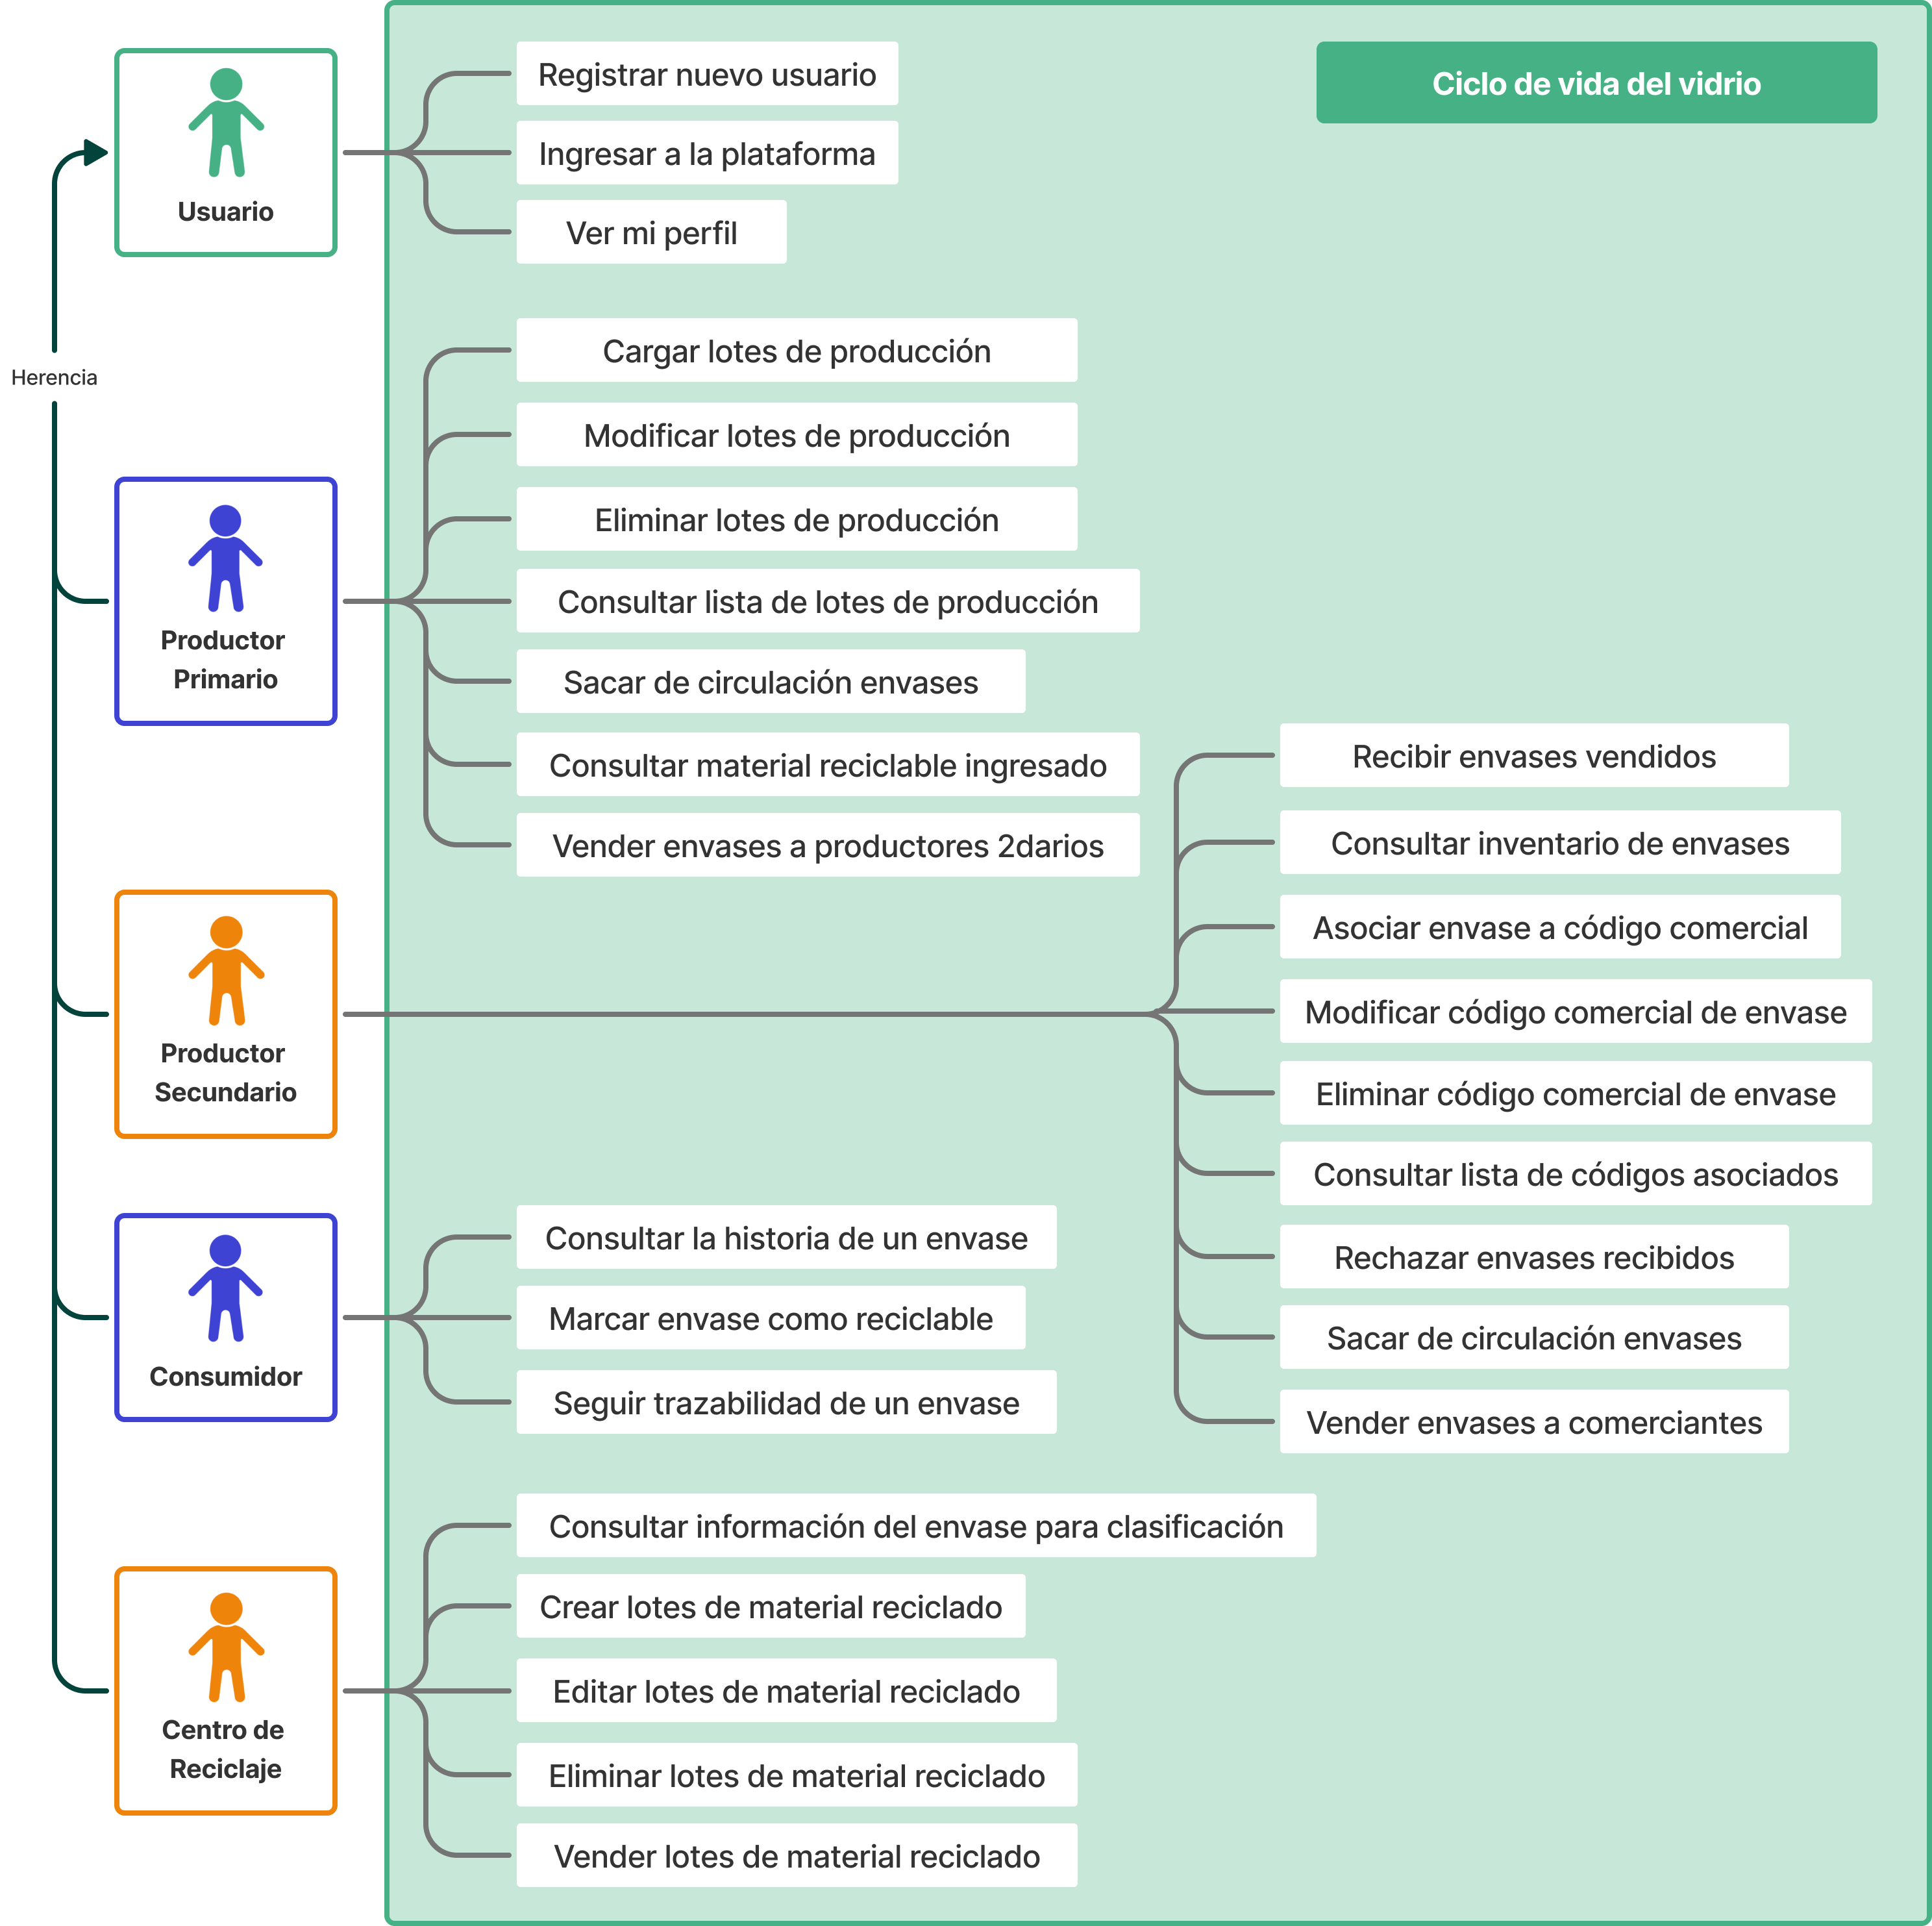
\includegraphics[width=\textwidth]{Figures/use-case-diagram.png}
    \caption{Diagrama de Casos de Uso del sistema de trazabilidad de vidrio}
    \label{fig:use-case-diagram}
\end{figure}

El diagrama muestra que cada actor tiene un conjunto de casos de uso alineado con sus responsabilidades. Por ejemplo, el Productor Primario puede registrar un nuevo lote de envases producidos o registrar la venta de envases a un Productor Secundario, mientras que el Productor Secundario puede consultar la \gls{trazabilidad} de origen de los envases recibidos y registrar su uso asociando los envases a un lote de producto final. Por otro lado, el Consumidor puede consultar el origen de un envase adquirido y el destino de un envase enviado a reciclaje, mientras que el Centro de Reciclaje puede recibir envases reciclables, consultar su composición de materiales y registrar su reciclaje. Los casos de uso de los diferentes actores se interrelacionan de manera cíclica, integrando la información de cada actor de la cadena en un único sistema de información interrelacionado que refleja el flujo de la \gls{economiacircular} de envases de vidrio. Por ejemplo, la acción ``Vender envases a productores secundarios'' del Productor Primario está ligada a los casos de uso del Productor Secundario, permitiendo rastrear el vidrio a lo largo de su ciclo de vida.

La lista de casos de uso sirve como punto de partida para la definición de los requerimientos funcionales y no funcionales del sistema, donde cada caso de uso se descompone en uno o más requerimientos específicos que describen las funcionalidades que el sistema debe implementar para cumplir con las expectativas de los actores.

\section{Definición de Requerimientos}
\label{sec:requirements-definition}

Después de identificar los casos de uso, se definen los requerimientos funcionales y no funcionales del sistema. Los requerimientos funcionales describen las funcionalidades específicas que el sistema debe ofrecer a los usuarios, mientras que los requerimientos no funcionales establecen las características de calidad que el sistema debe cumplir, tales como rendimiento, seguridad o usabilidad.

Los requerimientos se documentan de manera estructurada, asignando un identificador único a cada requerimiento para su seguimiento durante las etapas posteriores de diseño, implementación y pruebas del sistema. La descripción de cada requerimiento incluye su propósito, las condiciones bajo las cuales se cumple y las dependencias con otros requerimientos. Un ejemplo de requerimiento funcional es que ``el sistema debe permitir al Productor de Vidrio registrar un nuevo lote de vidrio, especificando la cantidad y el tipo de vidrio'', mientras que un requerimiento no funcional puede ser que ``el sistema debe garantizar la seguridad de los datos del usuario mediante autenticación y autorización''.

A partir de los casos de uso previamente identificados, se definieron 28 requerimientos funcionales y 6 requerimientos no funcionales para el sistema. Estos requerimientos se documentan en la etapa de modelado para su posterior seguimiento durante el desarrollo. Se establecen dependencias entre ellos, lo que permite identificar restricciones en el orden de implementación de las funcionalidades del sistema. Por ejemplo, el registro de un lote de vidrio (RF-006) es una dependencia para que dicho lote pueda ser recibido por un productor secundario para envasar productos (RF-016). La Tabla \ref{tab:functional-requirements} presenta los requerimientos funcionales, mientras que la Tabla \ref{tab:non-functional-requirements} muestra los requerimientos no funcionales definidos para el prototipo de trazabilidad de envases de vidrio basado en blockchain.

\begin{xltabular}{\textwidth}{@{} L{1.5cm} L{2.5cm} Y L{1.5cm} @{}}
	\caption{Requerimientos Funcionales del sistema de trazabilidad de envases de vidrio}
	\label{tab:functional-requirements}\\
	\toprule
	\textbf{ID} & \textbf{Título} & \textbf{Descripción} & \textbf{Deps.} \\
	\midrule
\endfirsthead

\toprule
\textbf{ID} & \textbf{Título} & \textbf{Descripción} & \textbf{Deps.} \\
\endhead

\multicolumn{4}{r}{\footnotesize Continúa en la siguiente página}
\\\bottomrule
\endfoot

\bottomrule
\endlastfoot
	RF-001 & Registrar usuarios & El sistema debe permitir registrar usuarios mediante un correo electrónico u otro medio con diferentes roles para hacer uso de las distintas partes del sistema. \par Los roles disponibles en esta primera etapa son: \par
  - Productor Primario \par
  - Productor Secundario \par
  - Consumidor \par
  - Reciclador. & - \\
	\hline
	RF-002 & Ingresar a la plataforma & Todos los usuarios deben poder ingresar a la plataforma con su correo electrónico registrado mediante algún método de autenticación, por ejemplo, con contraseña. & RF-001 \\
	\hline
	RF-003 & Mantener sesión de usuario & Cada cuenta de usuarios debe poder mantener abiertas múltiples sesiones en simultaneo. El usuario debe poder cerrar una sesión individual en cualquier dispositivo. La sesión debe mantenerse abierta en el dispositivo a lo largo del tiempo a pesar de que se cierre el navegador o aplicación. & RF-002 \\
	\hline
	RF-004 & Validar Autorización & Cada rol de usuario debe tener ciertos permisos y un usuario con un rol dado no debe poder realizar acciones que requieran un permiso del que no goza. Detalle:\par - Productor Primario: crear, editar, consultar y eliminar envases.\par - Productor Secundario: editar, consultar y eliminar productos. \par - Consumidor: consultar composición de productos \par - Reciclador: consultar composición de productos, crear, editar, consultar y eliminar lotes de reciclaje. & RF-002 \\
	\hline
	RF-005 & Ver mi perfil de usuario & Cada usuario debe poder consultar la información personal asociada a su cuenta y modificar algunos datos: Email, Nombre Empresa/persona (modificable), Responsable (modificable), Nro teléfono (modificable), Dirección pública blockchain. & RF-002 \\
	\hline
	RF-006 & Cargar lotes de producción & El productor puede cargar lotes de producción de envases de vidrio incluyendo la siguiente información: Cantidad de envases, Peso por envase, Color, Composición, Espesor, entre otras. & RF-004 \\
	\hline
	RF-007 & Editar lotes de producción & El productor puede editar la información de producción en caso de error hasta antes de comercializar el lote. & RF-006 \\
	\hline
	RF-008 & Eliminar lotes de producción & El productor puede eliminar un lote en caso de error hasta antes de comercializar el lote. & RF-006 \\
	\hline
	RF-009 & Consultar historial de producción & El productor puede consultar información histórica de todos los lotes que ha creado con sus detalles y puede consultar su \gls{trazabilidad} posterior. & RF-006 \\
	\hline
	RF-010 & Consultar material reciclable ingresado & El productor puede ver la lista de los lotes o conjuntos de materiales reciclables que volvieron a ingresar a su fábrica (como compra a la recicladora o devoluciones desde bodegas). & RF-006, RF-018, RF-025 \\
	\hline
	RF-011 & Sacar de circulación envases & El productor puede marcar grupos de botellas de un lote como fuera de circulación o enviado a reciclar (en caso de rotura, falla o desaparición). & RF-006 \\
	\hline
	RF-012 & Vender envases a productores secundarios & El productor puede marcar cierta cantidad de envases del lote como vendidos a un productor secundario específico. Los envases dejan de ser propiedad del productor y ya no puede modificarlos ni revenderlos. & RF-006 \\
	\hline
	RF-013 & Asociar envase a código comercial & El productor secundario puede asociar un código de barras (u otro tipo de código visible en la etiqueta impresa de su producto, como QR) a conjuntos de botellas compradas. \textbf{El código debe garantizar unicidad}. & RF-012 \\
	\hline
	RF-014 & Modificar código comercial & El productor secundario puede editar la información de códigos asociados a envases hasta antes de vender el producto. & RF-013 \\
	\hline
	RF-015 & Eliminar código comercial & El productor secundario puede eliminar códigos asociados a envases hasta antes de vender el producto. & RF-013 \\
	\hline
	RF-016 & Consultar inventario de envases nuevos & El productor secundario puede ver la lista de conjuntos de envases que ha comprado pero aún no ha utilizado (no han sido asociados a ningún producto propio ni código). El productor puede confirmar conformidad o rechazar la compra. & RF-012 \\
	\hline
	RF-017 & Rechazar envases recibidos & El productor secundario puede desconocer la transacción de transferencia de envases desde el productor en caso de no reconocer la compra o realizar una devolución por algún tipo de error. & RF-012 \\
	\hline
	RF-018 & Sacar de circulación envases & El productor secundario puede devolver botellas en caso de no conformidad, fallas de fábrica o rotura. Estos envases pueden transferirse al productor como material reciclable o descartarse. & RF-012 \\
	\hline
	RF-019 & Consultar historial de producción & El productor secundario puede consultar el historial de sus productos embotellados o botellas utilizadas. A su vez puede consultar su trazabilidad posterior a la comercialización. & RF-013 \\
	\hline
	RF-020 & Vender envases a comerciantes & El productor secundario puede marcar sus productos embotellados como vendidos al comerciante. & RF-013 \\
	\hline
	RF-021 & Consultar la historia de un envase & Mediante el código asociado a la botella, el ciudadano debe poder consultar el origen, composición y trazabilidad histórica de envase cualesquiera. & RF-013 \\
	\hline
	RF-022 & Marcar envase como reciclable & El ciudadano puede registrar un envase como ingresado al sistema de reciclaje escaneando su código. & RF-013 \\
	\hline
	RF-023 & Dar seguimiento a envases & El ciudadano puede hacer seguimiento del destino y trazabilidad hasta la disposición final de todos los envases que ingresó al sistema de reciclaje. & RF-022 \\
	\hline
	RF-024 & Consultar información del envase para clasificación & El reciclador clasificador puede escanear el código de la botella y obtener información relevante sobre su composición para su correcta clasificación. & RF-013 \\
	\hline
	RF-025 & Crear lotes de material reciclado & El reciclador puede crear lotes de material reciclado a partir de un conjunto de envases reciclables recibidos de los ciudadanos. Cada lote tiene los siguientes atributos: Peso, Dimensión (si aplica), Material, Composición. & RF-022 \\
	\hline
	RF-026 & Editar lote de material reciclado & El reciclador puede editar la información de un lote en caso de error hasta antes de su comercialización. & RF-025 \\
	\hline
	RF-027 & Eliminar lote de material reciclado & El reciclador puede eliminar un lote en caso de error hasta antes de su comercialización. & RF-025 \\
	\hline
	RF-028 & Vender lote de material reciclado & El reciclador puede marcar un lote de material reciclable como vendido a un productor y debe especificar el comprador. Se asume en este caso que el material fue efectivamente reciclado, finalizando la trazabilidad. & RF-025 \\
\end{xltabular}

\begin{xltabular}{\linewidth}{@{} L{1.5cm} L{2.5cm} Y @{}}
	\caption{Requerimientos No Funcionales del sistema de trazabilidad de envases de vidrio}
	\label{tab:non-functional-requirements}\\
	\toprule
	ID & Título & Descripción \\
	\midrule
\endfirsthead

\toprule
ID & Título & Descripción \\
\endhead

\multicolumn{3}{r}{\footnotesize Continúa en la siguiente página}
\\\bottomrule
\endfoot

\bottomrule
\endlastfoot
RNF-01 & Transparencia & La trazabilidad de un producto debe ser libremente accesible por cualquier usuario autenticado del sistema en todo momento. \\
\hline
RNF-02 & Disponibilidad & El sistema debe estar disponible para su uso 24/7 \\
\hline
RNF-03 & Escalabilidad & El sistema debe soportar un número creciente de transacciones \\
\hline
RNF-04 & Mantenibilidad & El sistema debe poder ser mantenible por otros desarrolladores de la industria actual en el futuro \\
\hline
RNF-05 & Interoperabilidad & El sistema debe ser integrable con múltiples sistemas de stock y gestión de terceros preexistentes \\
\hline
RNF-06 & Integridad & Los datos de trazabilidad no deben poder ser alterados luego de cargados sin dejar registro público de la modificación \\
\end{xltabular}

La lista de requerimientos funcionales y no funcionales sirve como base para la siguiente fase de modelado, en la que se definirán las historias de usuario y se planificará el desarrollo del sistema. A su vez, la lista de requerimientos se utilizará posteriormente en la validación y verificación del sistema, asegurando que todas las funcionalidades implementadas cumplan con las expectativas y necesidades de los usuarios.

% TODO: why a big space is rendered here?

\section{Historias de Usuario y Planificación}
\label{sec:user-stories}

A partir de la definición de los requerimientos funcionales y no funcionales del sistema, se procede a la creación de las historias de usuario. Las historias de usuario permiten documentar las funcionalidades del sistema desde la perspectiva de sus actores, utilizando un formato estandarizado que describe el rol, la acción deseada y el beneficio esperado: ``Como [rol], quiero [acción], para [beneficio]''. Por ejemplo, ``Como Productor Primario, quiero poder editar la información de un lote de envases antes de su comercialización, para poder corregir cualquier error en los datos de producción y asegurar la precisión en el registro''. Esta forma de documentar requerimientos facilita la priorización de funcionalidades y la comprensión de las necesidades desde un enfoque centrado en el usuario a la hora de desarrollar el sistema.

Cada historia de usuario se complementa con criterios de aceptación que establecen las condiciones necesarias para su validación, vinculándose directamente con uno o más requerimientos previamente definidos. Esta trazabilidad entre los requerimientos y las historias de usuario es un mecanismo de control que guía el proceso de desarrollo y asegura que la implementación cumpla con las expectativas planteadas. En el contexto del modelo en V, las historias de usuario establecen la base para la fase de pruebas de aceptación, garantizando que el sistema final se alinee con los objetivos del proyecto.

A continuación se presenta un ejemplo de historia de usuario con sus respectivos criterios de aceptación, que ilustra la relación entre las funcionalidades y las necesidades de los actores.

\begin{center}
\fbox{
  \begin{minipage}{0.95\linewidth}
    \vspace{0.3cm}
    \textbf{Historia de Usuario:} Consultar historial de producción de lotes de envases de vidrio \\
    \textbf{Como} productor, \\
    \textbf{Quiero} poder consultar el historial de todos los lotes de producción con sus detalles y trazabilidad, \\
    \textbf{Para} poder revisar la información de producción y rastrear cada lote en su ciclo de vida.
    
    \vspace{0.5cm}
    
    \textbf{Criterios de Aceptación:}
    \begin{enumerate}
      \item \textbf{Visualización del historial de lotes:}
      \begin{itemize}
        \item El sistema debe mostrar una lista de todos los lotes creados por el productor con la siguiente información:
        \begin{itemize}
          \item \textbf{Código de lote}
          \item \textbf{Fecha de producción}
          \item Cantidad de envases
          \item Peso por envase
          \item Color
        \end{itemize}
      \end{itemize}
      
      \item \textbf{Acceso a detalles de cada lote:}
      \begin{itemize}
        \item Al seleccionar un lote específico, el sistema debe mostrar los detalles completos, incluyendo:
        \begin{itemize}
          \item Espesor
          \item \textbf{Fecha de producción}
          \item Observaciones adicionales
        \end{itemize}
      \end{itemize}
    \end{enumerate}
    \vspace{0.3cm}
  \end{minipage}
}
\end{center}

En el presente trabajo, se definieron un total de 28 historias de usuario, donde cada historia de usuario se corresponde exactamente con un requerimiento funcional del sistema. Los requerimientos no funcionales se abordan de manera transversal, asegurando que aspectos como el rendimiento, la seguridad y la usabilidad sean considerados en el diseño e implementación del sistema.

Cada historia de usuario se registró en la herramienta de gestión Jira \footnote{\url{https://www.atlassian.com/es/software/jira}}, con el objetivo de facilitar la gestión del proceso de desarrollo siguiendo la metodología Kanban. Como parte del proceso de planificación, se estimó el esfuerzo necesario para implementar la funcionalidad de cada historia de usuario y se registró en la herramienta Jira junto con la tarea correspondiente. La estimación del esfuerzo consideró la complejidad técnica, el tiempo requerido proyectado para implementarlo y las interdependencias entre las funcionalidades, lo que permitió una planificación objetiva del desarrollo.

La planificación del proyecto se realizó mediante un diagrama de Gantt \footnote{\url{https://www.atlassian.com/es/agile/project-management/gantt-chart}}. Un diagrama de Gantt es una herramienta visual que muestra la secuencia de las tareas, sus dependencias y los plazos de implementación estimados. Este diagrama permite visualizar el cronograma del proyecto, facilitando la identificación de hitos y la gestión de recursos. En este caso, se utilizó para planificar las historias de usuario y su implementación en iteraciones o sprints, asegurando que todas las funcionalidades necesarias sean contempladas y ejecutadas de manera ordenada según sus dependencias.

En la Figura \ref{fig:jira-board}, se muestra una captura del tablero utilizado para el seguimiento del progreso de cada historia de usuario en la plataforma Jira, mientras que la Figura \ref{fig:gantt-chart} presenta el diagrama de Gantt creado para este proyecto. Con la planificación armada, se estimó que el desarrollo del sistema tendría una duración de 6 semanas, con un total de 28 historias de usuario a implementar. Esta estimación de tiempo corresponde exclusivamente al tiempo de codificación de funcionalidades del prototipo, ya que, posterior a la etapa de generación de código, se procede a la fase de codificación y ejecución de pruebas automatizadas y validación manual del sistema, donde es posible a su vez que se deban realizar ajustes o correcciones de programación en función de los resultados obtenidos.

\begin{figure}[!htb]
  \centering
  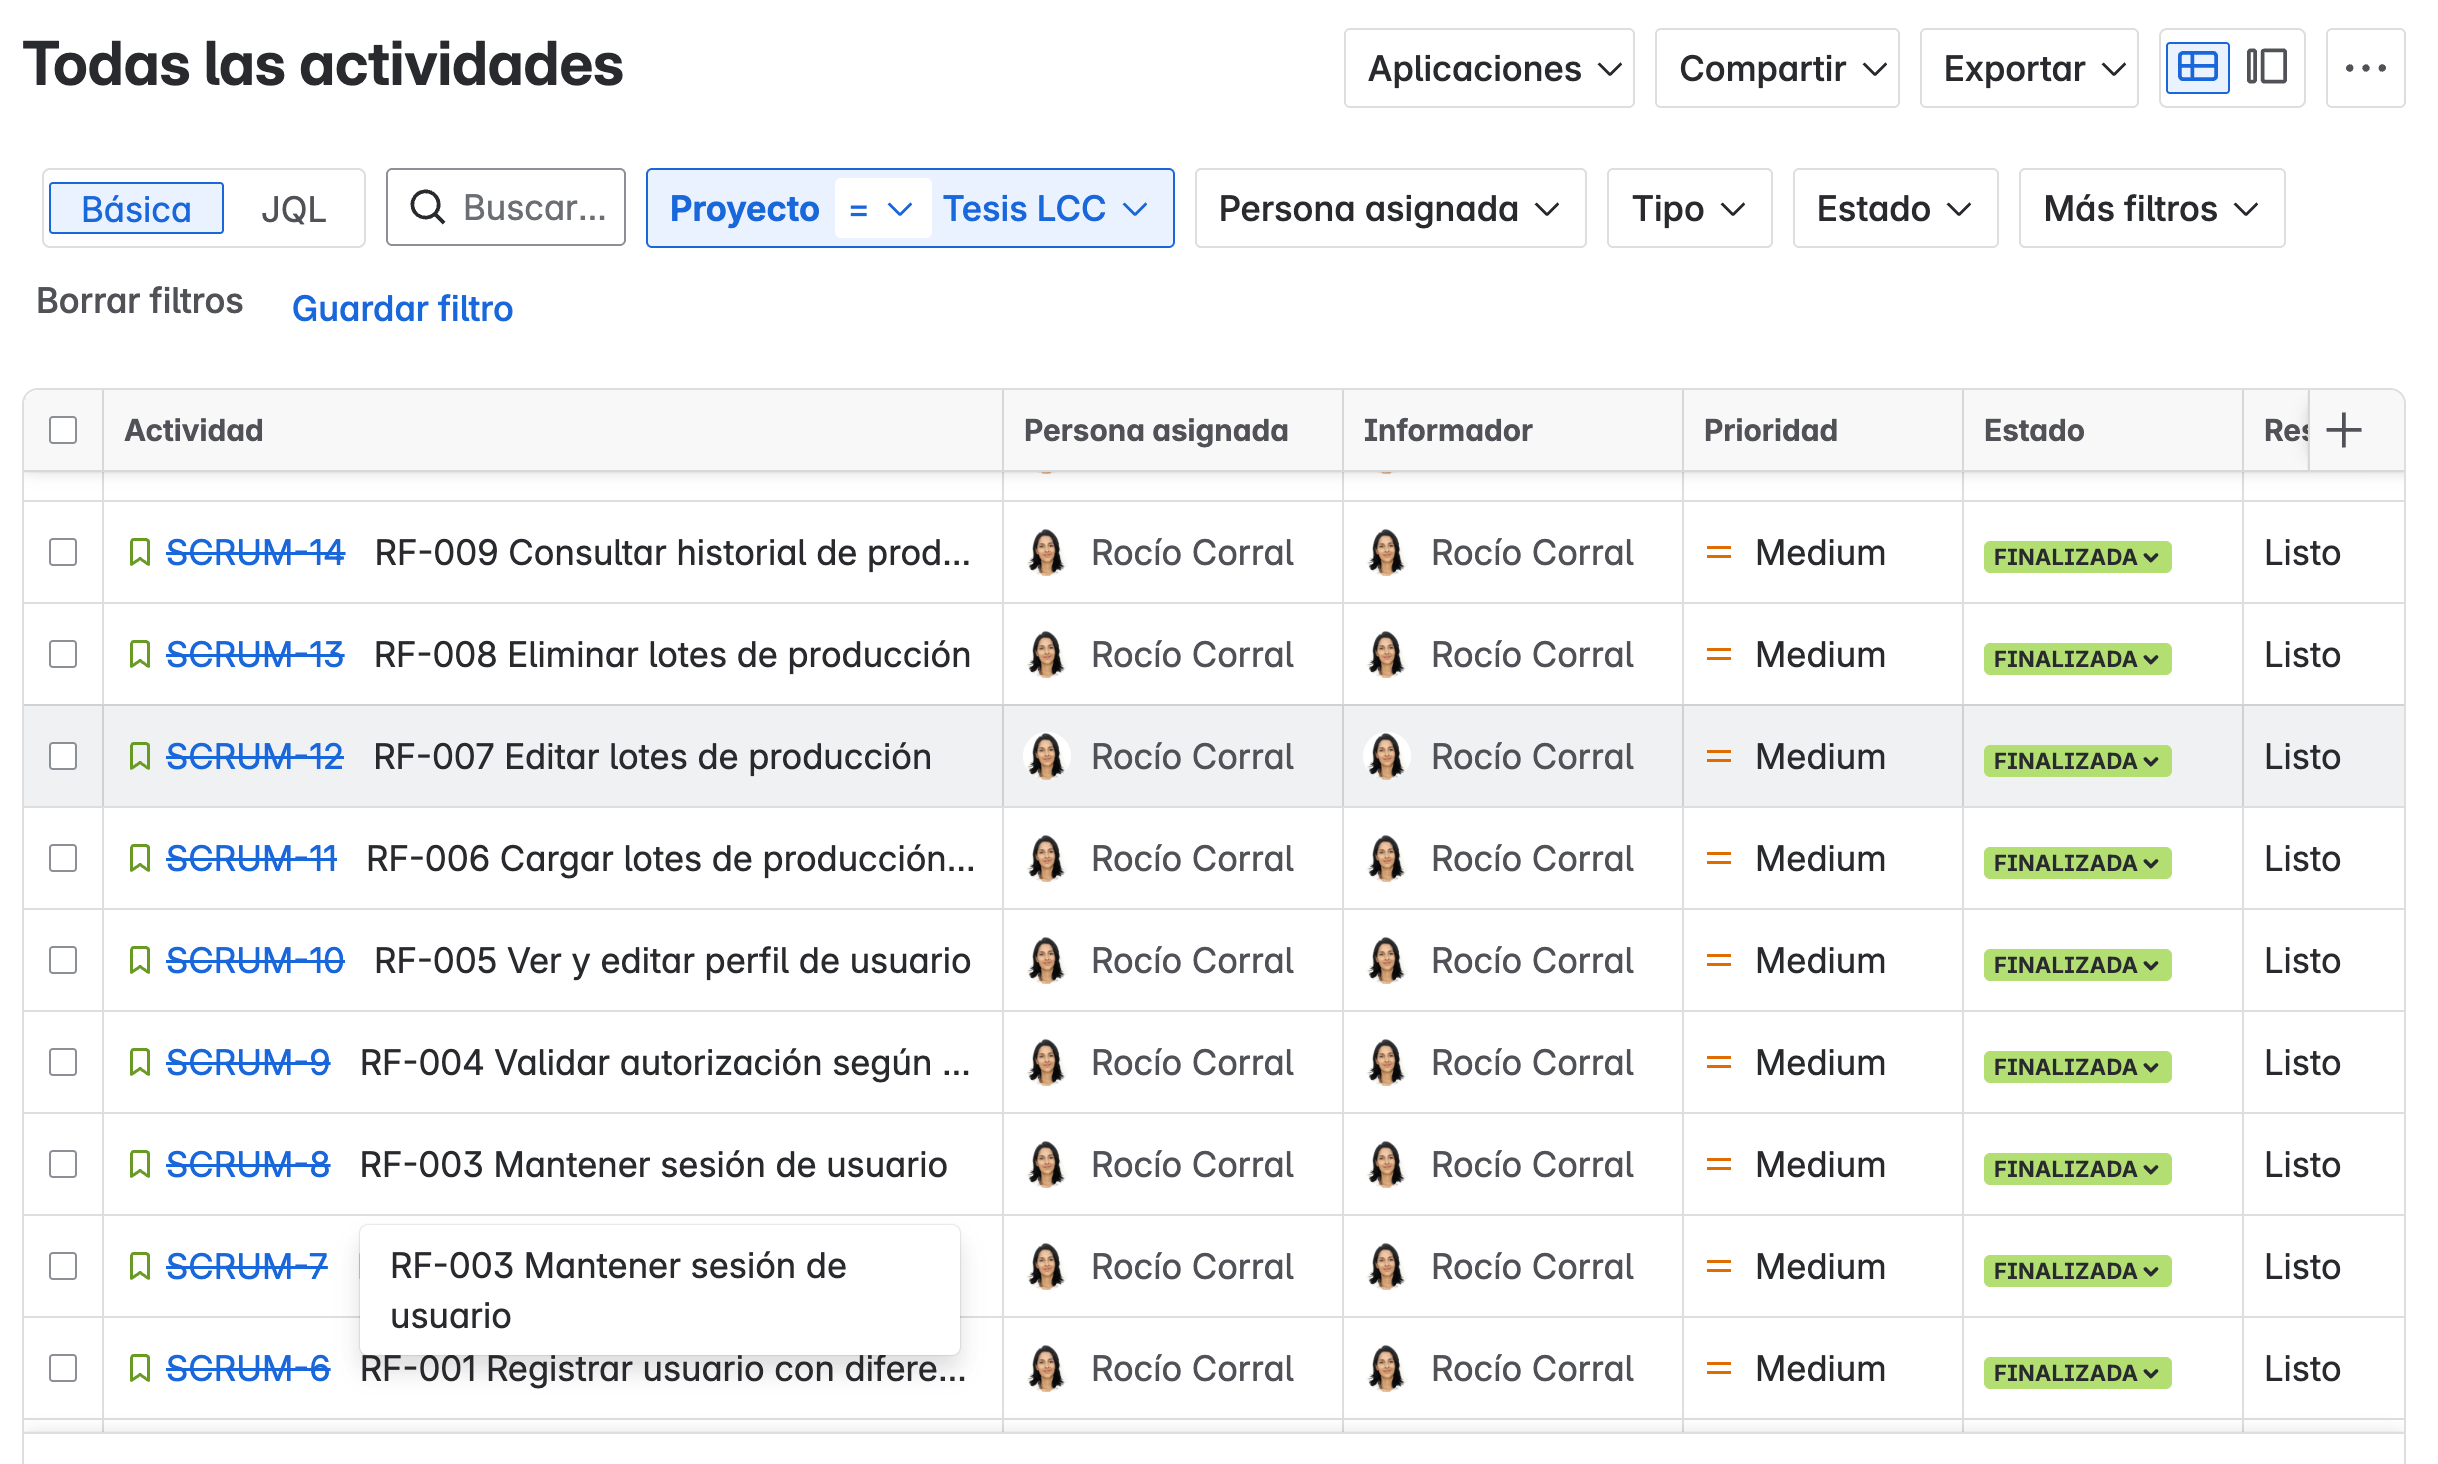
\includegraphics[width=\textwidth]{Figures/jira-board.png}
  \caption{Tablero de Jira para la gestión de historias de usuario}
  \label{fig:jira-board}
\end{figure}

\begin{figure}[!htb]
  \centering
  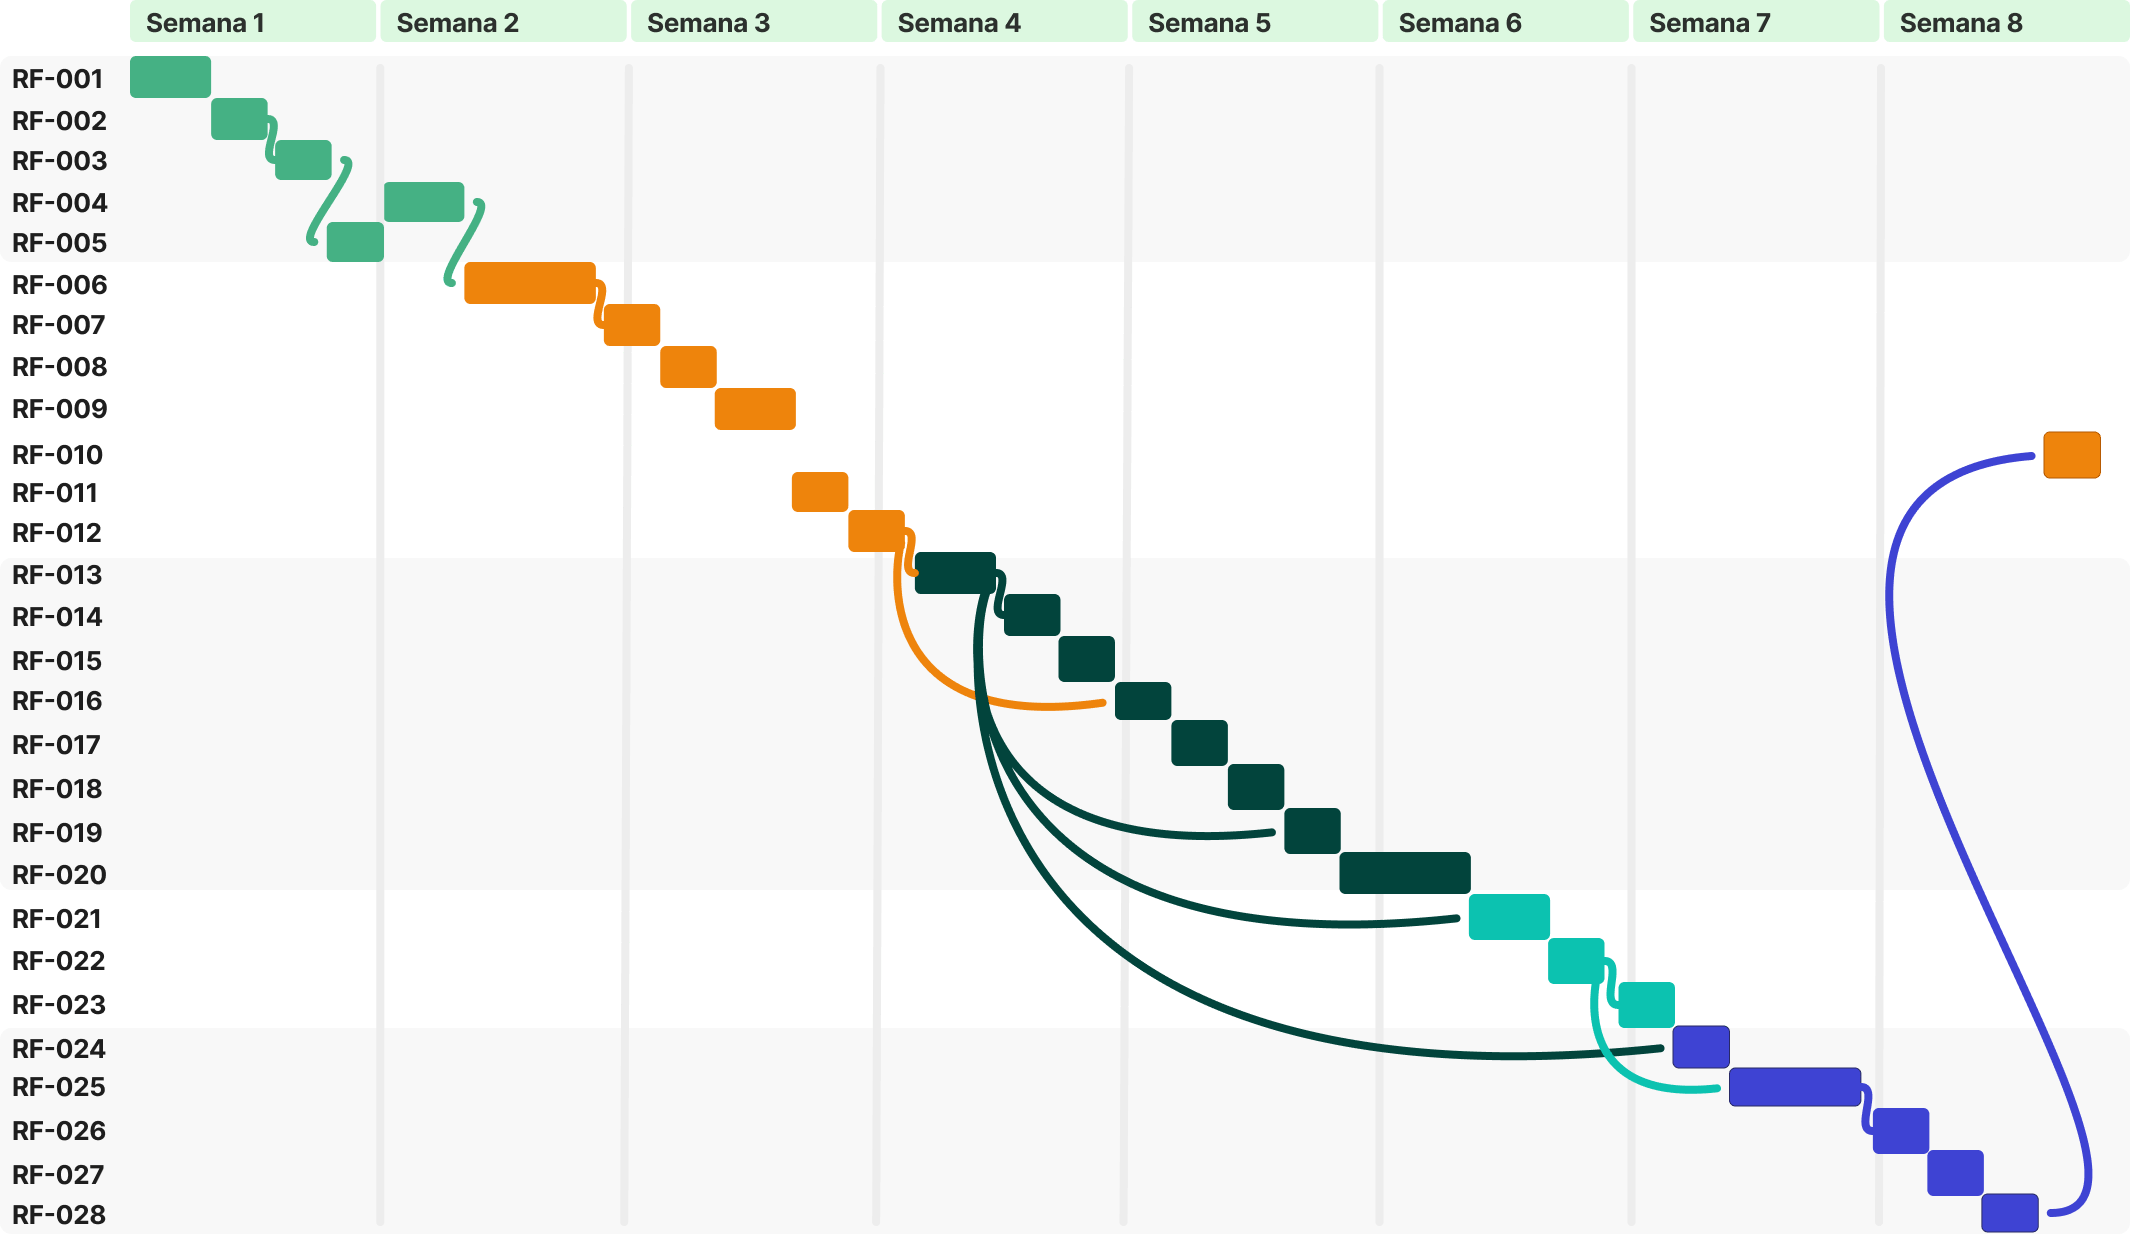
\includegraphics[width=\textwidth]{Figures/gantt-chart.png}
  \caption{Diagrama de Gantt para la planificación del proyecto}
  \label{fig:gantt-chart}
\end{figure}

Concluidas las fases de modelado de requerimientos y planificación, se establece la base para la siguiente etapa del proceso. El conjunto de requerimientos, casos de uso y la planificación detallada con las historias de usuario constituyen la referencia que guiará las fases de diseño, implementación y pruebas del sistema. En el próximo capítulo, se abordará el diseño de la arquitectura y los componentes del sistema, donde se definirán las soluciones tecnológicas y la estructura del software que implementará los requerimientos establecidos.
